\documentclass[aspectratio=169,t]{beamer}
\usepackage[utf8]{inputenc}
\usepackage[T1]{fontenc}
\usepackage[english]{babel}
\usepackage{hyperref}
\usepackage{tikz}

\usepackage{graphicx}
\usepackage{epstopdf}
\usepackage{multirow}

\usepackage{psfrag}
\usepackage{pgfplots}
\usepackage{framed}
\usepackage{xcolor}
\usepackage{booktabs}
\usepackage{caption}
\usepackage{epstopdf}
\usepackage{amsmath}
\usepackage{tabularx}
\usepackage[]{bookmark}
%\usepackage[3D]{movie15}
%\usepackage{media9}
\usepackage[binary-units,abbreviations]{siunitx}
\usepackage[textfont=normalsize, labelfont=normalsize, justification=centering]{subcaption}
\usepackage{marvosym}
\usepackage{calc}
\usepackage{color, colortbl}
\usepackage[]{svg} 
\usepackage[]{trfsigns} 
\usepackage[nomessages]{fp}
\usepackage[]{csquotes}\MakeOuterQuote{"}
\selectcolormodel{rgb}

\makeatletter
\def\beamer@calltheme#1#2#3{\def\beamer@themelist{#2}
	\@for\beamer@themename:=\beamer@themelist\do
	{\usepackage[{#1}]{\beamer@themelocation/#3\beamer@themename}}}
\def\usefolder#1{\def\beamer@themelocation{#1}}
\def\beamer@themelocation{}
\usefolder{theme}

\usetikzlibrary{matrix,
	decorations.pathreplacing,
	calc,
	positioning,
	external,
	3d,
	shapes,
	arrows,
	pgfplots.statistics}
\pgfplotsset{compat=1.16}
\tikzstyle{faunode}=[rounded corners, draw=faublue, fill=faublue!10,  align=center, inner sep=0.3cm, line width=0.4mm]
\tikzstyle{fauellipseFixedWidth}=[ellipse, draw=faublue, fill=faublue!10,  align=center, inner sep=0.3cm, line width=0.4mm, minimum width=3cm]
\tikzstyle{fauellipse}=[ellipse, draw=faublue, fill=faublue!10,  align=center, inner sep=0.3cm, line width=0.4mm]
\tikzstyle{fauarrow}=[draw=faublue,->, line width=0.4mm]
\tikzstyle{fauline}=[draw=faublue, line width=0.4mm]


\usepackage[backend=bibtex,sorting=none,doi=true,style=phys]{biblatex}
%\usepackage[]{biblatex}
\bibliography{./references}

% Themes:
%  - fau:          FAU theme
%  - fau-tf:       TechFak FAU theme
%  - fau-tf-lme:   TechFak LME FAU theme
%
% Options:
%  - image:        Cover image on title page
%  - plain:        Plain title page
%  - longtitle:    Title page layout for long title
\usetheme[longtitle]{fau-tf-lme}

% END of THEME SETTINGS
% --------------------------------------------------------------------------------------------------------------------------------------------------------------------------

\sisetup{
exponent-product =\ensuremath{{\,\cdot\,}}
}

% Enable semi-transparent animation preview
\setbeamercovered{transparent}
\setbeamertemplate{blocks}[rounded]
\captionsetup{labelformat=empty,labelsep=none, labelfont=normalsize, justification=centering}


\newcommand\Wider[2][1.0cm]{%
\makebox[\linewidth][c]{%
  \begin{minipage}{\dimexpr\textwidth+#1\relax}
  \raggedright#2
  \end{minipage}%
  }%
}


\let\origitem\item
\renewcommand{\item}{\normalfont\origitem}
\newcommand{\bluefat}[1]{\textcolor{faublue}{\textbf{#1}}}
\newcommand{\bolditem}{\normalfont\origitem\bfseries}
\newcommand{\question}{{\bf Question: }}
\newcommand{\answer}{{\bf Answer: }}
\newcommand{\myExample}{{\bf Example }}
\newcommand{\real}{\mbox{${\mathbb R}$}}
\definecolor{defColor}{rgb}{0.8,0.87,0.97}
\definecolor{defColorT}{rgb}{0,0,0}
\definecolor{defColorF}{rgb}{1,1,1}
\newenvironment{myDefinition}{%
	\def\FrameCommand{\fboxsep=\FrameSep{} \fcolorbox{defColorF}{defColor}}%
	\color{defColorT}\MakeFramed{\FrameRestore{}}}%
{\endMakeFramed}

% Title page
\title[Medical Engineering II]{Medical Engineering - Imaging Systems}
\author{Prof.\ Dr.-Ing.\ habil.\ Andreas Maier}
\date{SS 2021}
\institute{Pattern Recognition Lab (CS 5)}

\newcommand{\password}{\texttt{mt2\_ss21}}


\AtBeginSection[]{
	{
		\setbeamertemplate{footline}{}
		\begin{frame}[noframenumbering]{\insertsubtitle}
			 \tableofcontents[currentsection]
		\end{frame} 
	}
}
\AtBeginSubsection[]{
	{

		\setbeamertemplate{footline}{}
		\begin{frame}[noframenumbering]{\insertsubtitle}
			 \tableofcontents[currentsection, currentsubsection]
		\end{frame} 
	}
}


\usepackage{transparent}

\usepackage{subcaption}
\usepackage{wrapfig}
\usepackage{bm}
\usepackage{ragged2e}

\def\mat#1{\ensuremath{\bm #1}}

\hypersetup{
    colorlinks=true,        % false: boxed links; true: colored links
    linkcolor=faublue,      % color of internal links (change box color with linkbordercolor)
    linktoc=none
}

\setbeamercovered{transparent}

\setbeamertemplate{frametitle continuation}[from second]
\setbeamertemplate{bibliography item}{\lower1.5pt\hbox{\pgfuseimage{beamericonarticle}}}

\usetikzlibrary{decorations.pathreplacing,calc}

\newcommand{\tikzmark}[1]{\tikz[overlay,remember picture] \node (#1) {};}
 

\DeclareMathOperator*{\argmin}{argmin}

\renewcommand{\vec}[1]{\boldsymbol{#1}}

%\title[\color{faugray} MT1: Computed Tomography]{Medical Engineering I:\\Computed Tomography}

\author[A.~Maier, O.~Taubmann, M.~Bögel, Y.~Xia]{Andreas Maier, Oliver Taubmann, Marco Bögel, Yan Xia, Stephan Seitz}
\subtitle{Spectral Computed Tomography}


\AtBeginSubsection[]{
    {

        %\setbeamertemplate{footline}{}
      %  \begin{frame}[noframenumbering]{\insertsubtitle}
      %      \large \tableofcontents[currentsection, currentsubsection]
     %   \end{frame} 
    }
}

\begin{document}

\frame[plain,c]{\titlepage} % plain-Option deaktiviert Kopf- und Fusszeile

\begin{frame}
	\frametitle{\insertsubtitle}

	%\tableofcontents[subsectionstyle=shaded]
	\tableofcontents
\end{frame}

\section{CT Measurement Process Reviewed}

\begin{frame}
    \frametitle{Hardware Setup}
    \begin{itemize}
        \item Classical fan beam geometry:
    \end{itemize}
    \begin{figure}
        \centering{}
        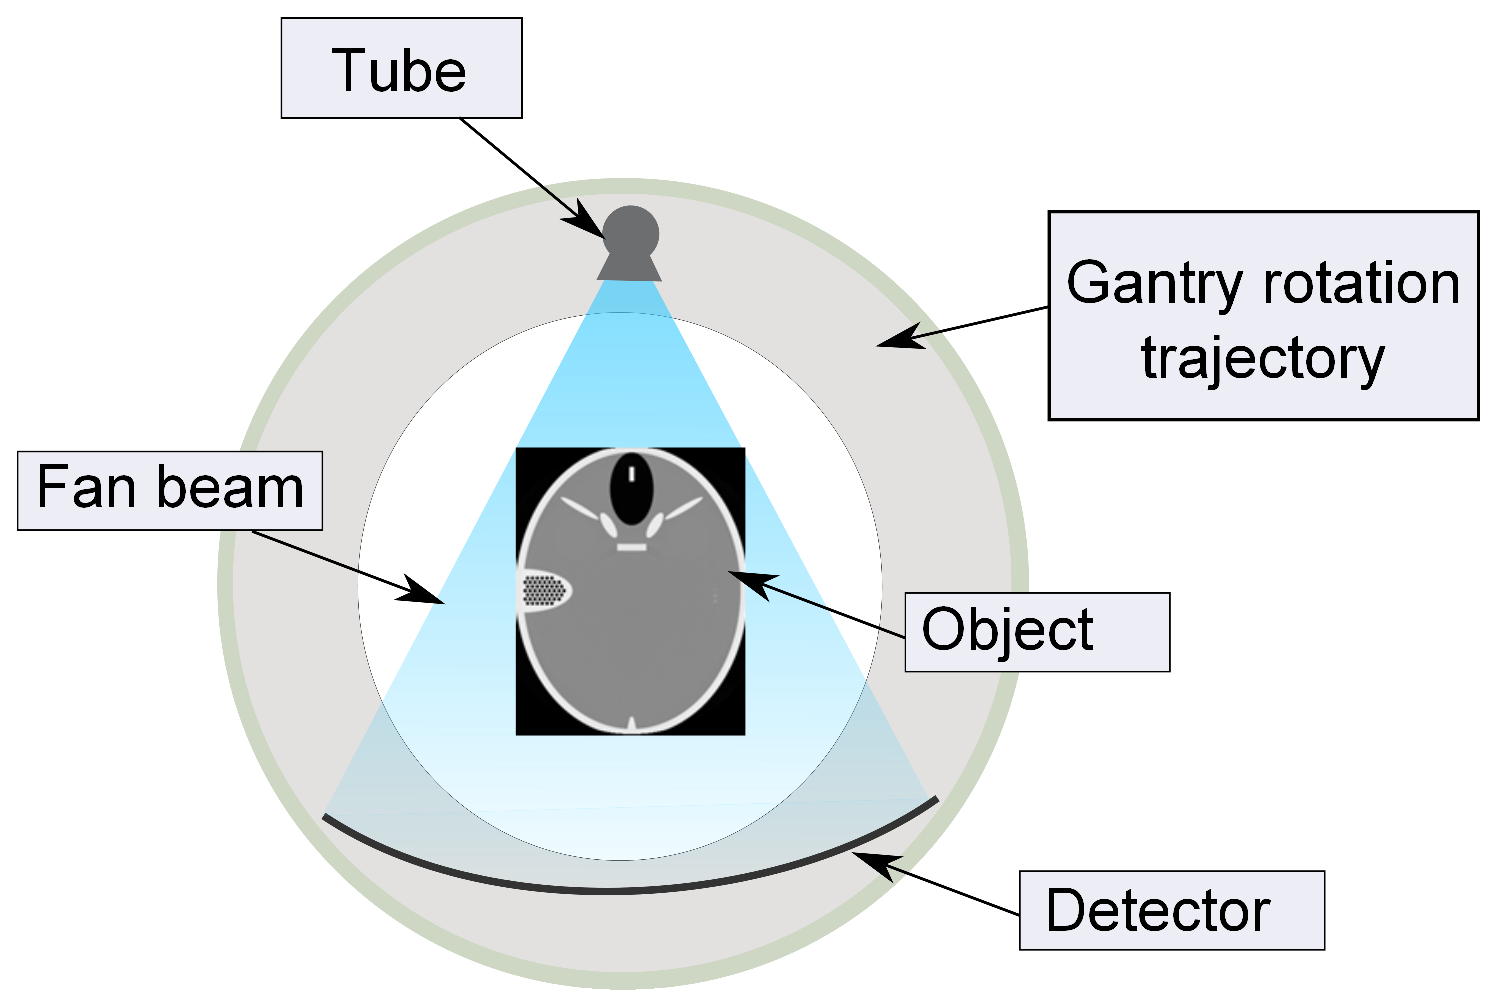
\includegraphics[scale=0.35]{images/multict.eps}
    \end{figure}
\end{frame}

\begin{frame}
    \frametitle{Sinogram}
    \begin{minipage}{0.52\textwidth}
        \begin{figure}
            \centering{}
            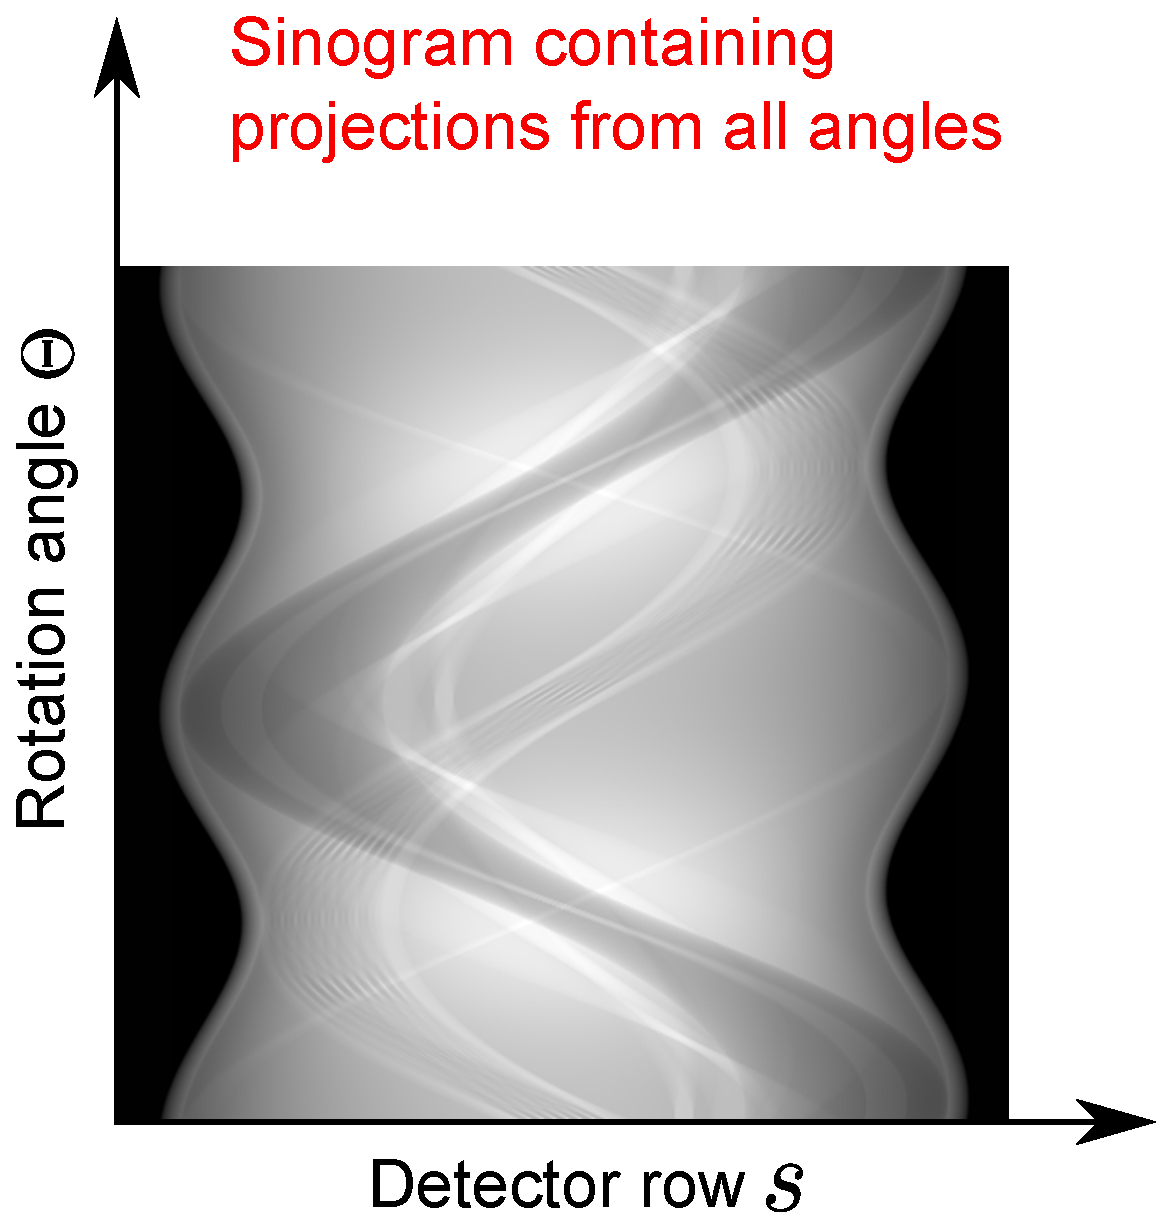
\includegraphics[scale=.30]{images/sinogram.eps}
        \end{figure}
    \end{minipage}
    \begin{minipage}{0.45\textwidth}
        \begin{figure}
            \centering{}
            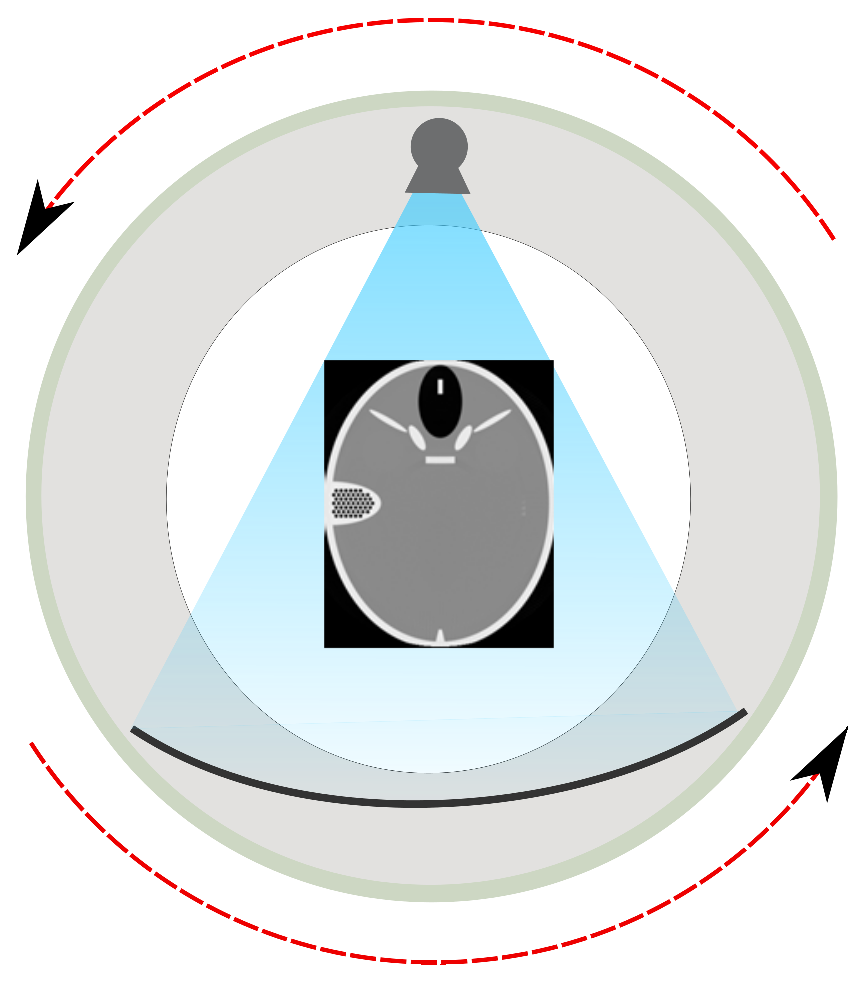
\includegraphics[scale=.35]{images/multict2.eps}
        \end{figure}
    \end{minipage}
\end{frame}

\begin{frame}{Projection Signal}

    \begin{columns}[c, onlytextwidth]
        \begin{column}{0.6\textwidth}
            Signal for single reading: \\
            \psfrag{ln}{{\LARGE $p(\Theta, s)$}}
            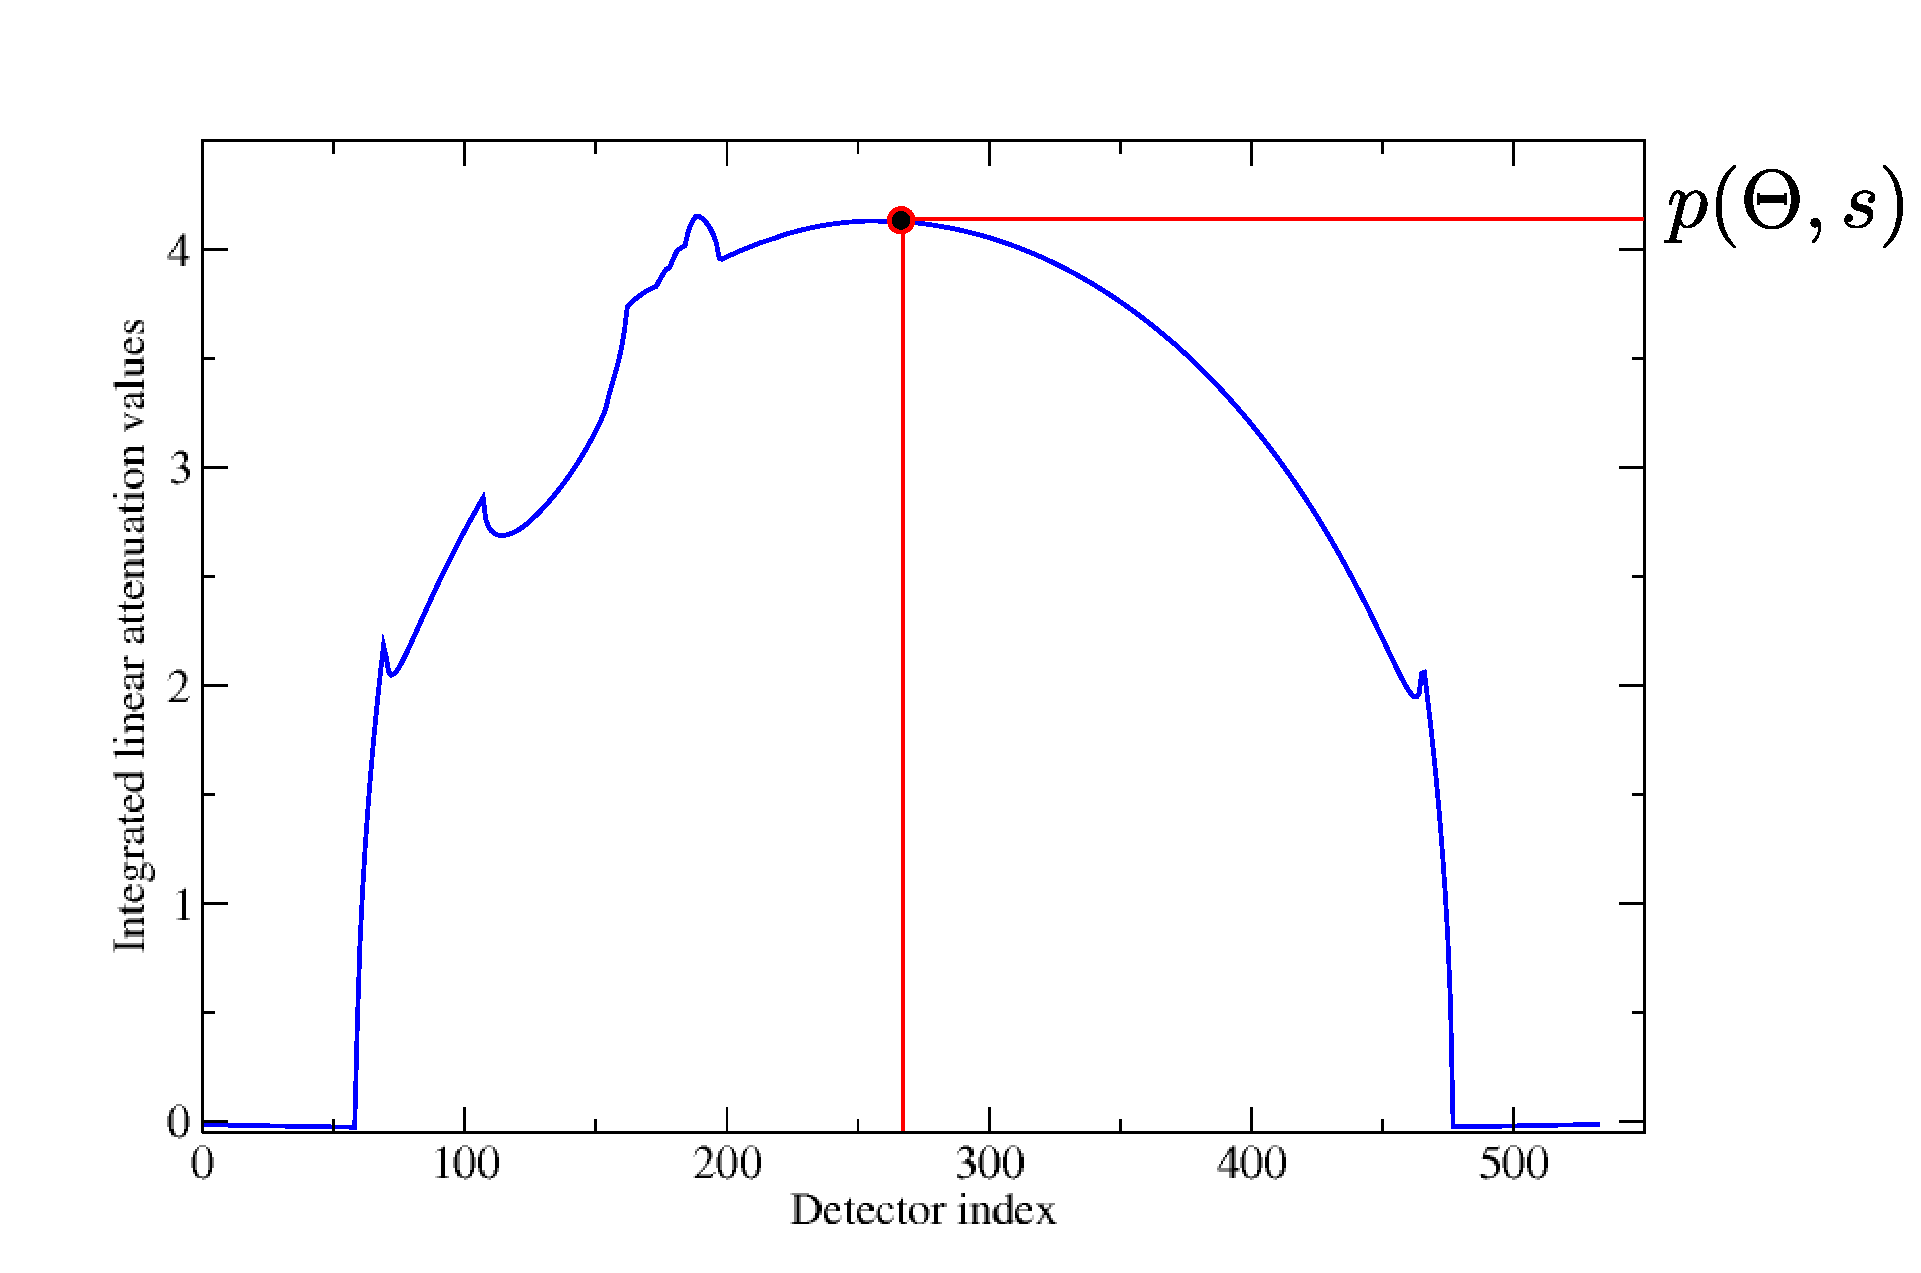
\includegraphics[width=0.8\textwidth]{images/projsig.eps}\\
            Measured intensity for a ray $l$:
            \begin{eqnarray*}
                p(\Theta, s) = \int{\mu}(l)dl
            \end{eqnarray*}
        \end{column}\begin{column}{0.4\textwidth}
            \begin{figure}
                \psfrag{l}{\LARGE{$\mu(l)$}}
                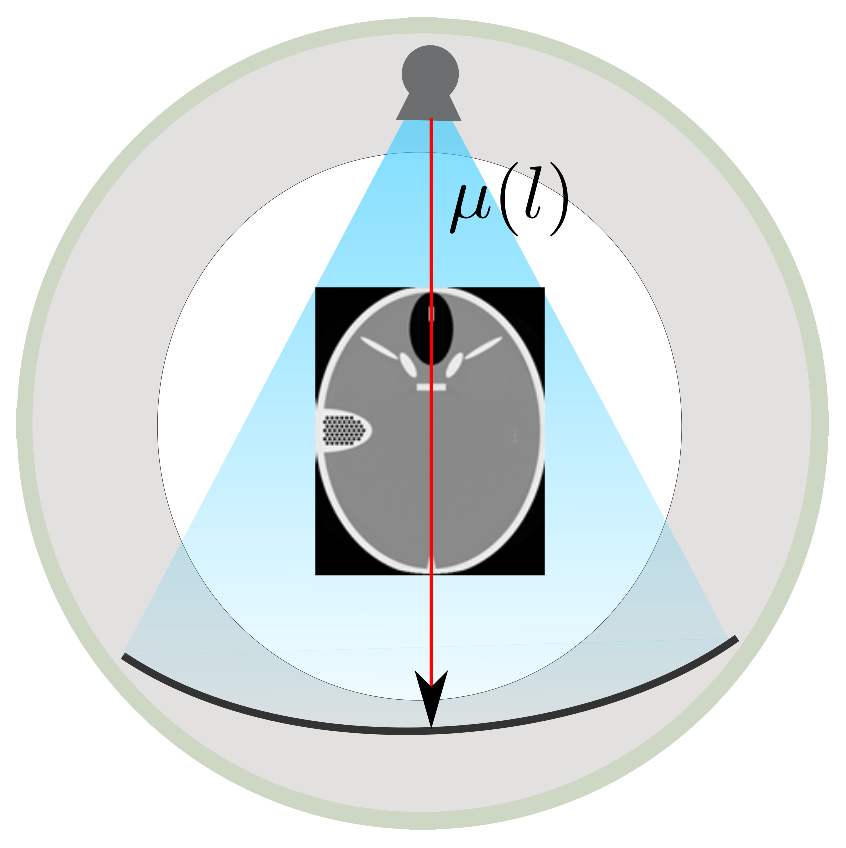
\includegraphics[width=0.8\textwidth]{images/multict3.eps}
            \end{figure}
        \end{column}
    \end{columns}
\end{frame}

\begin{frame}{Attenuation Law}
    \begin{align*}
        p^{\star}(\Theta, s)                               & = I_0 \cdot \exp\left(-\int	\mu(l)dl\right) \\
        -\ln\left(\dfrac{p^{\star}(\Theta, s)}{I_0}\right) & = p(\Theta, s) \tag{Radon transform}
    \end{align*}
    \begin{itemize}
        \item $p^{\star}(\Theta, s)$ denotes the measured X-ray intensity
        \item $I_0$ is the measured X-ray intensity without any attenuator
        \item $\mu(\vec x)$ is the \textit{linear attenuation coefficient} of the object at location $\vec x = (x ,y)$
        \item Reconstruction of $\mu(\vec x)$ from projections $p(\Theta, s)$\\ (e.\,g.\ by Iterative Reconstruction or Filtered Backprojection)
    \end{itemize}
\end{frame}


\section{X-ray Attenuation with Polychromatic Radiation}

\begin{frame}[c]{Monoenergetic vs. Polyenergetic Attenuation}
    \begin{itemize}
        \setlength\itemsep{0.4cm}
        \item \textbf{Problem:} The previous formula only holds for monoenergetic X-ray sources
        \item X-ray tubes for medical CT have a continuous X-ray spectrum
        \item Sources for monoenergetic radiation like synchrotrons or radioactive elements are not suitable for medical CT
        \item \textbf{Traditional solution:} Apply standard reconstruction methods and correct for resulting \textit{beam hardening artifact}
    \end{itemize}
\end{frame}

\begin{frame}
    \frametitle{X-ray Attenuation Physics}
    \begin{figure}
        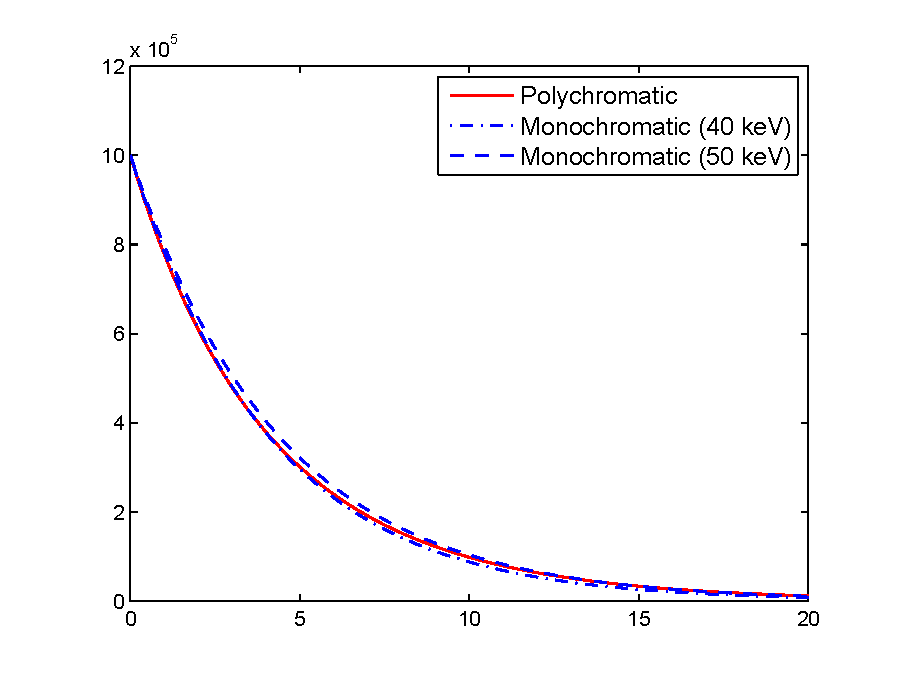
\includegraphics[height=0.6\textheight]{images/phxray1.eps}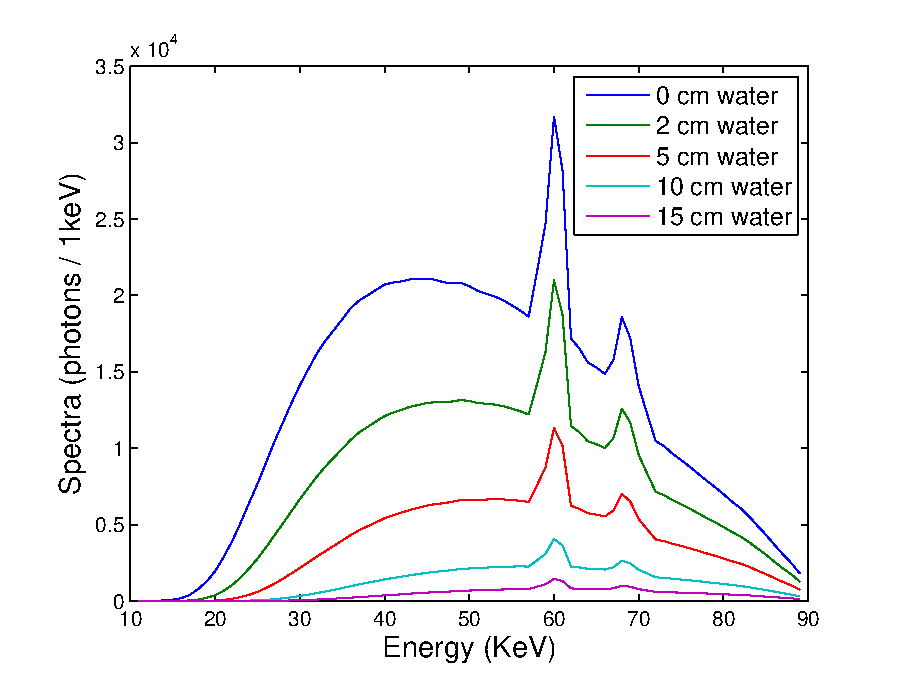
\includegraphics[height=0.6\textheight]{images/phxray2.eps}\\
    \end{figure}
    \begin{itemize}
        \item Mass attenuation is a function of energy
        \item Observation: Attenuation causes beam hardening in continuous X-ray spectra, as low energy components are attenuated stronger
    \end{itemize}
\end{frame}

\begin{frame}[c]{Beam Hardening}
        \vspace{-0.5cm}
    \begin{columns}[c, onlytextwidth]
        \begin{column}{0.6\textwidth}
            \bluefat{Consequence:}

            \begin{itemize}
                \item Standard reconstruction methods underestimate attenuation when beam hardening takes place
            \end{itemize}

            \vspace{1.0cm}
            \bluefat{Beam hardening correction:}

            \begin{itemize}
                \setlength\itemsep{0.3cm}
                \item Replace measured attenuation with an effective water length
                \item Effective water lengths for several attenuation values measured in calibration step

            \end{itemize}
            \vspace{-1.0cm}
        \end{column}\begin{column}{0.4\textwidth}
            \begin{figure}
                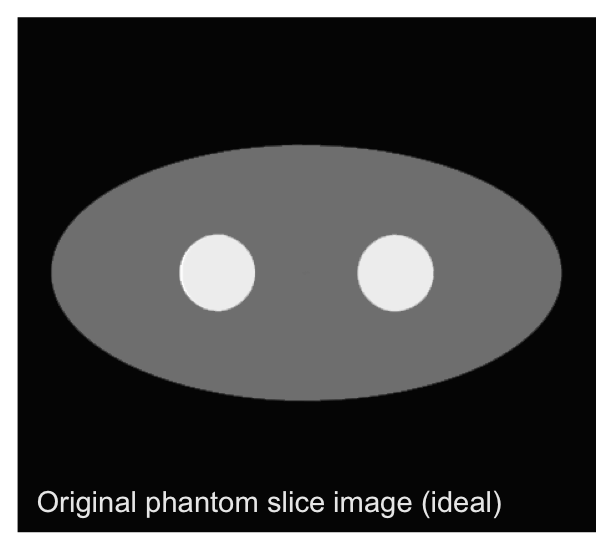
\includegraphics[height=0.45\textheight,clip=true,trim=0 0 0 30]{images/beam1.eps}\\
                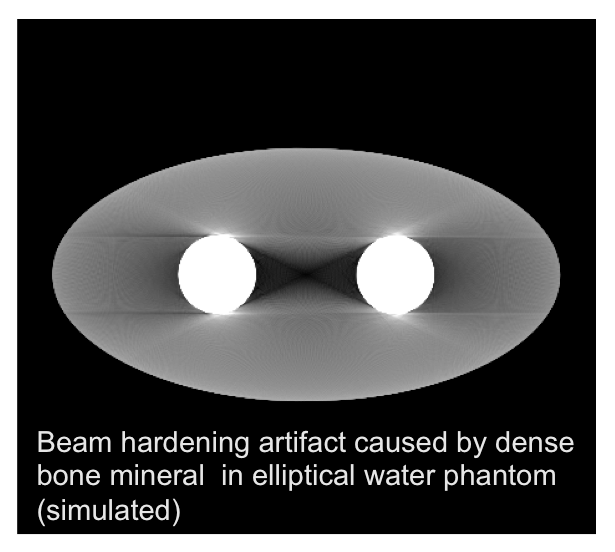
\includegraphics[height=0.45\textheight,clip=true,trim=0 0 0 30]{images/beam2.eps}
            \end{figure}
        \end{column}
    \end{columns}
\end{frame}


\section{Basics of Spectral CT Algorithms}

\begin{frame} [c]{Spectral CT}
    \begin{itemize}
        \setlength\itemsep{0.4cm}
        \item Effective water lengths do not determine scanned materials quantitatively
        \item Spectral CT computes the \textit{spectral attenuation coefficient} (mass attenuation times density) from multiple measurements at different energy weightings
        \item Different energy weightings can be achieved by varying the tube spectrum S(E) and/or the detector energy sensitivity D(E)
    \end{itemize}
\end{frame}

\begin{frame}[c]{Polychromatic Version of the Attenuation Law}
    \begin{itemize}
        \item The attenuation law for polychromatic radiation reads:
              \begin{eqnarray*}
                  p^{\star}_{\text{PC}}(\Theta,s) = \int S(E)D(E) \cdot \exp\left(-\int \mu(E, l)dl\right)dE
              \end{eqnarray*}
        \item This cannot be solved directly for $\mu(E,x)$ using standard reconstruction methods
        \item In the energy range of medical CT from 20 to 150 keV, the mass attenuation coefficient of body materials is dominated by two physical attenuation phenomena:
              \begin{itemize}
                  \item Incoherent (Compton) scatter
                  \item Photoelectric effect
              \end{itemize}
        \item The spectral attenuation coefficient of a body material can be expressed as a linear combination of two basis functions
    \end{itemize}
\end{frame}

\begin{frame}[c]{Polychromatic Version of the Attenuation Law}
    \begin{figure}
        \begin{centering}
            \includegraphics[width=0.5\linewidth]{images/PolychromaticModel.pdf}\caption{\label{fig:Poly}A spectrum and the integral under it.}
            \par\end{centering}
    \end{figure}
\end{frame}




\section{Measurement Concepts}

\begin{frame}[c]{How to Measure at Multiple Spectral Weightings?}
    \begin{itemize}
        \setlength\itemsep{0.4cm}
        \item For most quantitative CT applications, multiple measurements at different energy weightings are required
        \item Several approaches to multi-energy measurements are either currently investigated or already commercially available
              \begin{itemize}
                  \item Dual-kVp measurements
                  \item kVp-switching
                  \item Dual Source CT
                  \item Dual Layer detectors
                  \item Counting detectors
              \end{itemize}
    \end{itemize}
\end{frame}

\begin{frame}
    \frametitle{Dual-kVp}
    \vspace{-0.3cm}
    \begin{itemize}
        \item Make multiple CT scans of the same object at different tube voltages
        \item \bluefat{Pro:} Can be done with a standard CT scanner
        \item \bluefat{Cons:} Slow, no movement allowed between scans, pratically not feasable for most scenarios in medical CT
    \end{itemize}
    %\begin{center}
    %\begin{tabular}{ccc}
    %\includegraphics[width=0.3\textwidth]{}               & 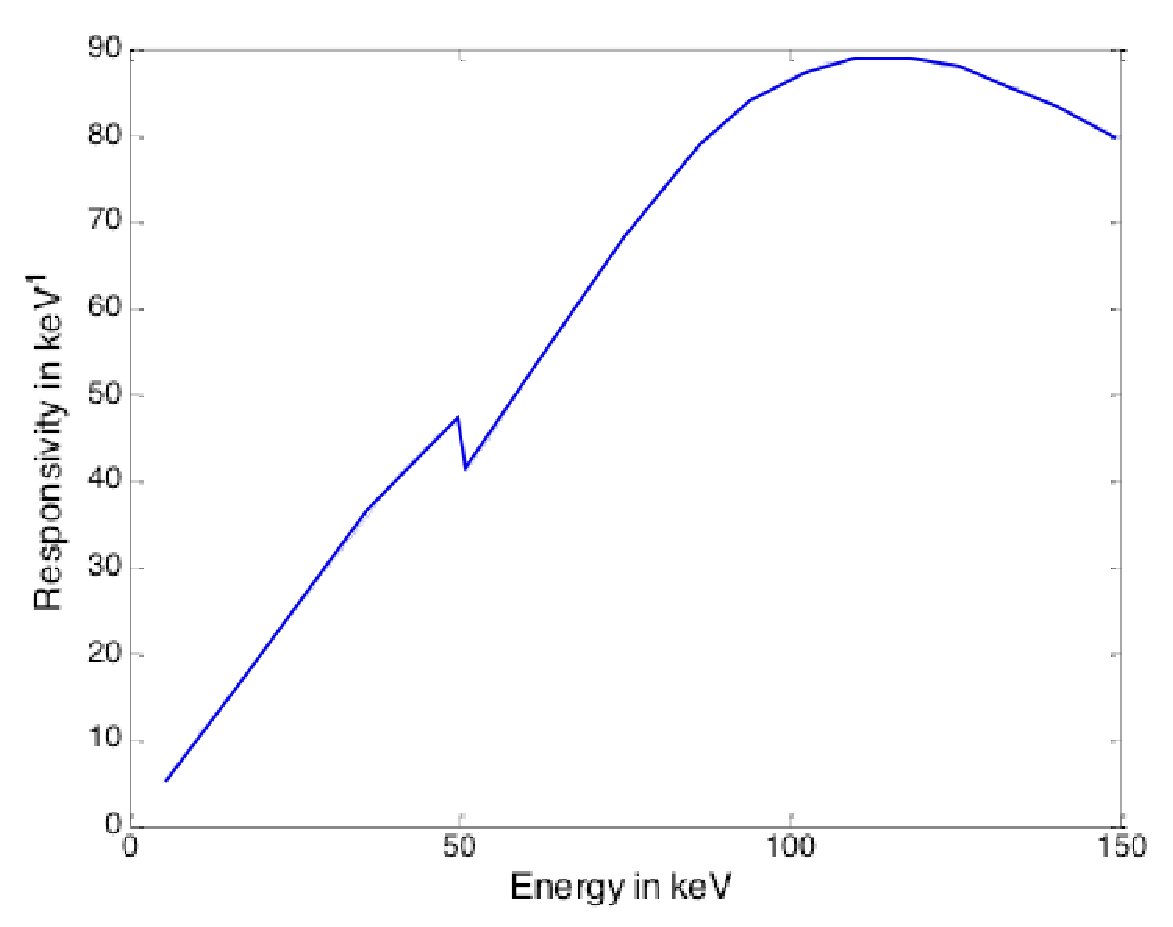
\includegraphics[width=0.3\textwidth]{images/dual2.eps}                   & 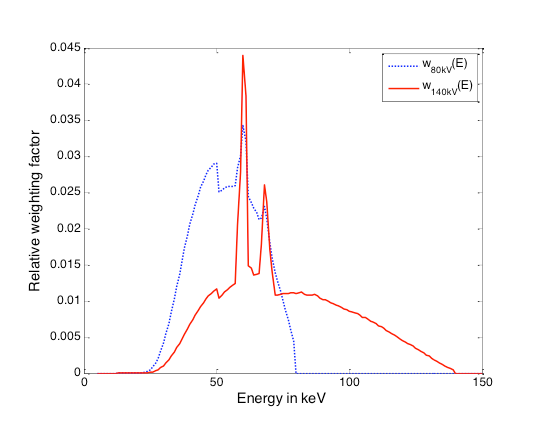
\includegraphics[width=0.3\textwidth]{images/dual3.eps}                                   \\
    %{ Normalized tube spectra$S(E)$ at \mbox{80 and 140 kVp}} & { Detector sensitivity $D(E)$ of a typical \mbox{CT detector}} & { Resulting system weighting functions \mbox{$\text{S(E)}\cdot\text{D(E)}$}}
    %\end{tabular}
    %\end{center}
    \begin{columns}[c, onlytextwidth]
        \begin{column}{0.33\textwidth}
            \begin{figure}[]
                \centering
                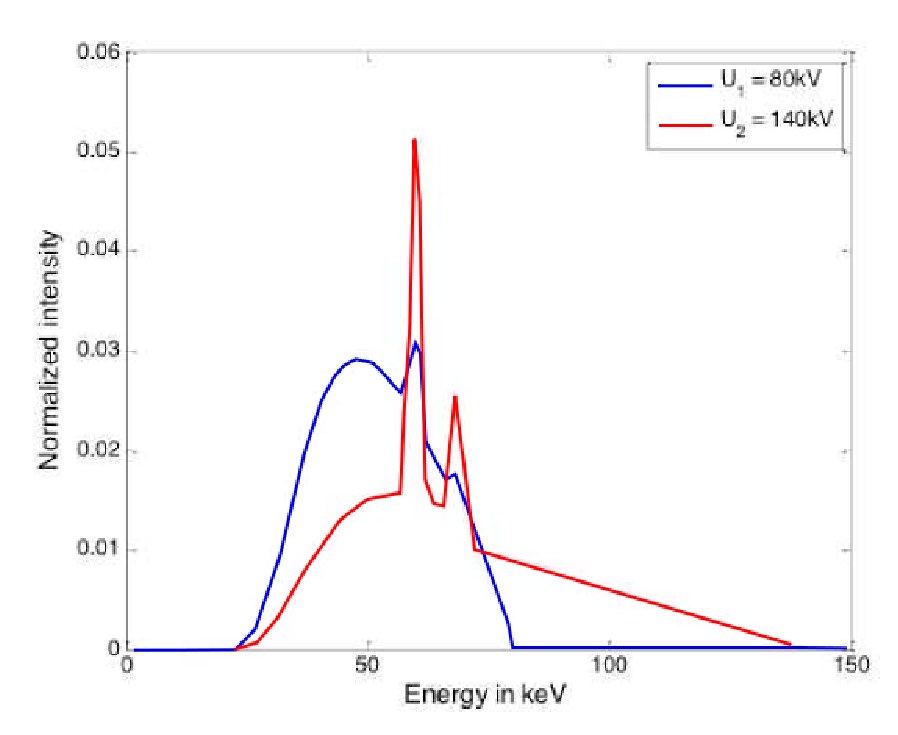
\includegraphics[width=\textwidth]{images/dual1.eps}
                \caption{Normalized tube spectra $S(E)$ at 80~and~140~kVp}%
                \label{fig:k}
            \end{figure}
        \end{column}\begin{column}{0.33\textwidth}
            \begin{figure}[]
                \centering
                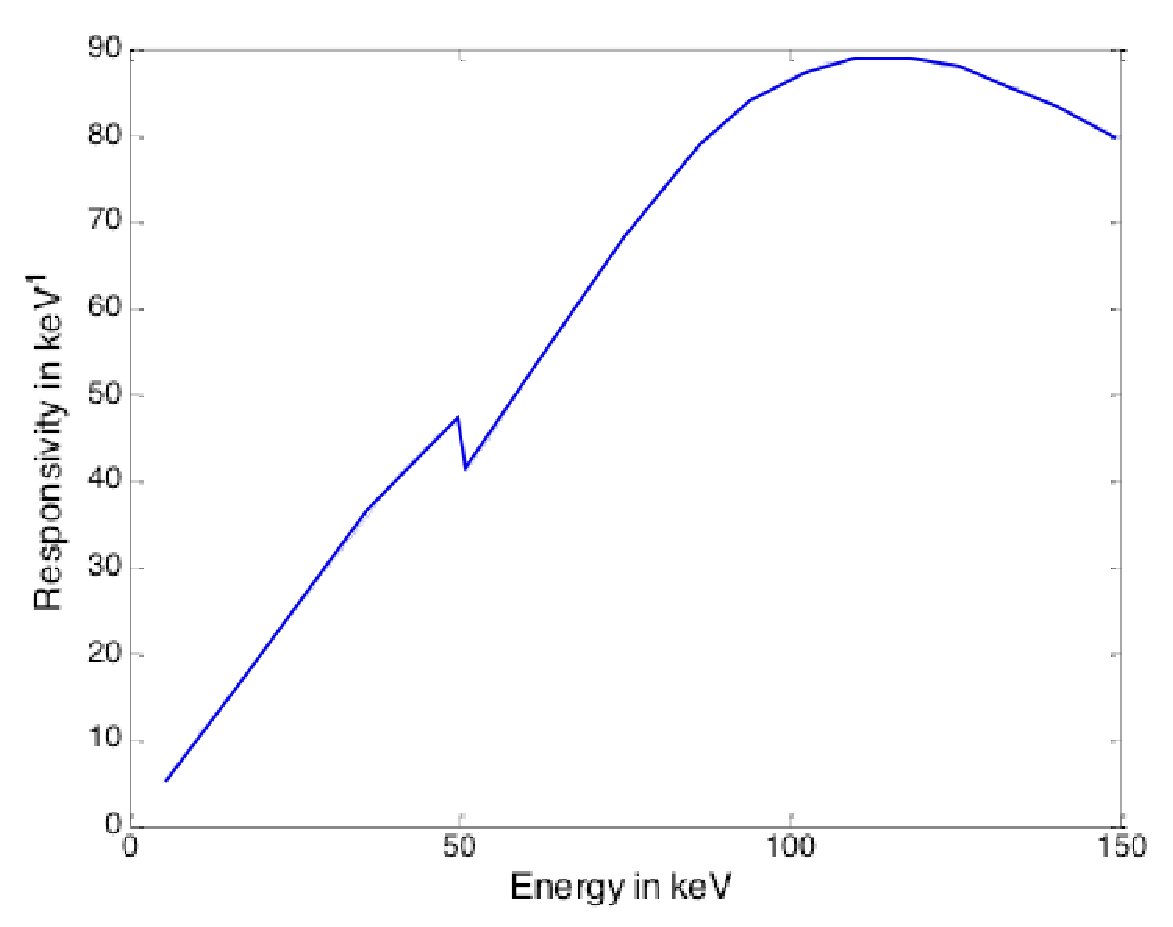
\includegraphics[width=\textwidth]{images/dual2.eps}
                \caption{Detector sensitivity $D(E)$ of a typical CT detector}
            \end{figure}
        \end{column}\begin{column}{0.33\textwidth}
            \begin{figure}[]
                \centering
                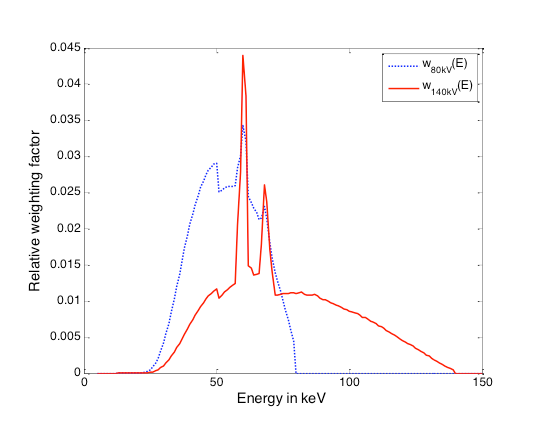
\includegraphics[width=\textwidth]{images/dual3.eps}
                \caption{Resulting system weighting functions $\text{S(E)}\cdot\text{D(E)}$}
            \end{figure}
        \end{column}
    \end{columns}
\end{frame}

\begin{frame}
    \frametitle{kVp-switching}
    \vspace{-0.3cm}
    \begin{itemize}
        \item Tube voltage is switched between readings of one scan
        \item \bluefat{Pros:} Fast, mostly standard equipment used
        \item \bluefat{Cons:} Readings at different weightings are not perfectly aligned, tube current cannot be adapted to kVp setting (dose!), very fast kVp switching capability of the tube required
    \end{itemize}
    \begin{columns}[c, onlytextwidth]
        \begin{column}{0.33\textwidth}
            \begin{figure}[]
                \centering
                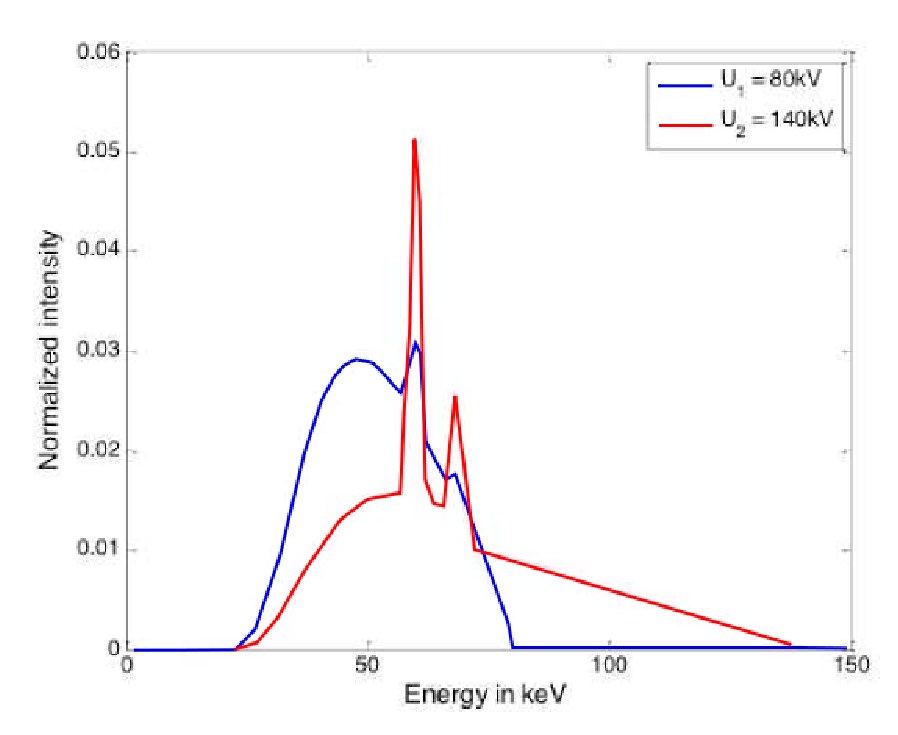
\includegraphics[width=\textwidth]{images/dual1.eps}
                \caption{Normalized tube spectra $S(E)$ at 80~and~140~kVp}
            \end{figure}
        \end{column}\begin{column}{0.33\textwidth}
            \begin{figure}[]
                \centering
                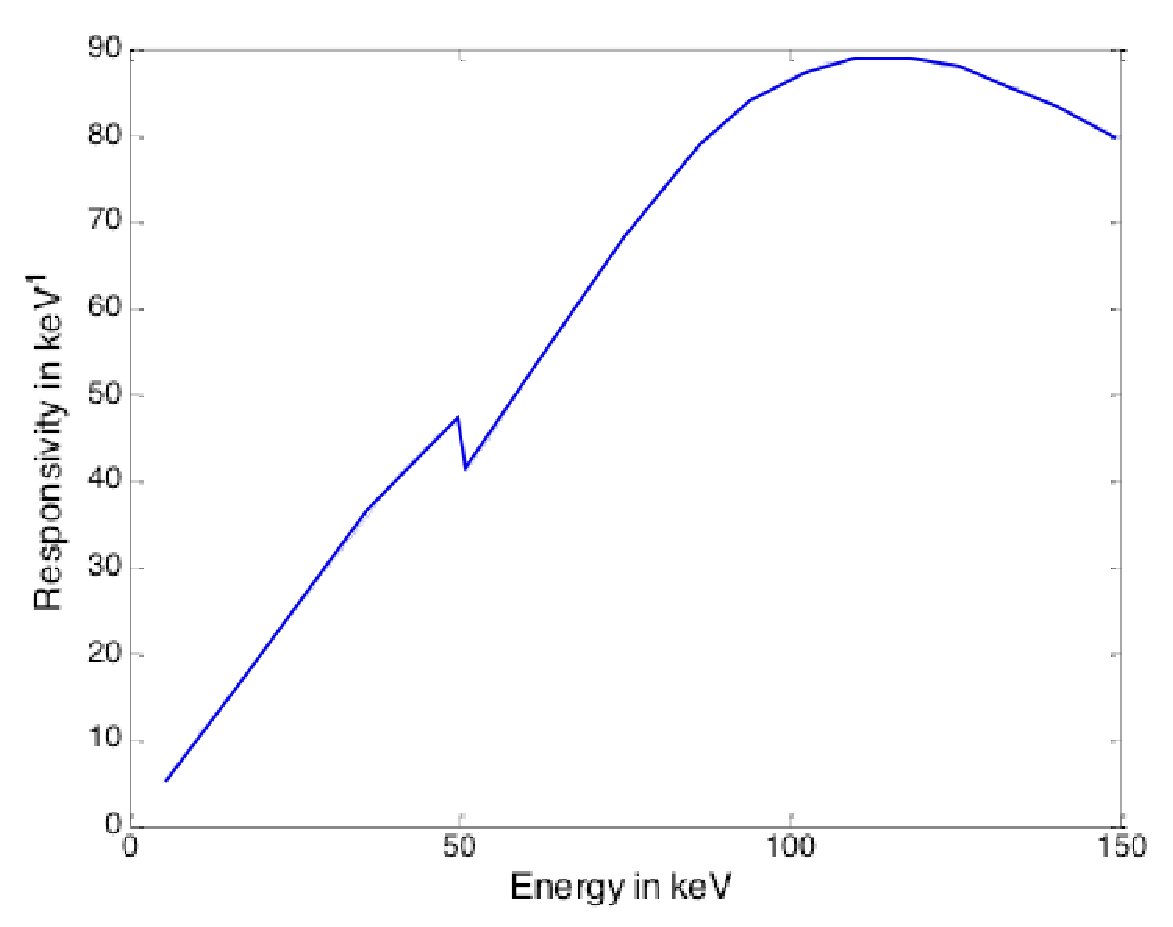
\includegraphics[width=\textwidth]{images/dual2.eps}
                \caption{Detector sensitivity $D(E)$ of a typical CT detector}
            \end{figure}
        \end{column}\begin{column}{0.33\textwidth}
            \begin{figure}[]
                \centering
                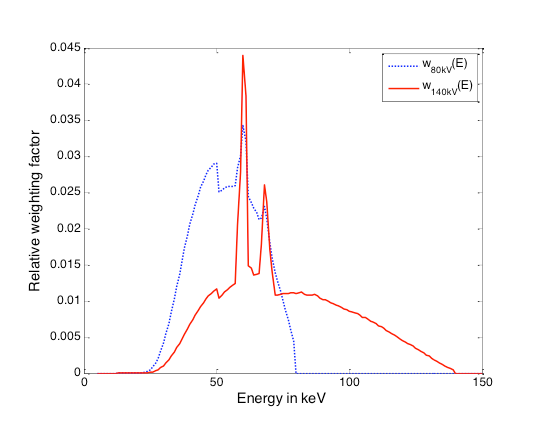
\includegraphics[width=\textwidth]{images/dual3.eps}
                \caption{Resulting system weighting functions $\text{S(E)}\cdot\text{D(E)}$}
            \end{figure}
        \end{column}
    \end{columns}%
    %\begin{center}
    %\begin{tabular}{p{7.5cm}p{7.5cm}p{7.5cm}}
    %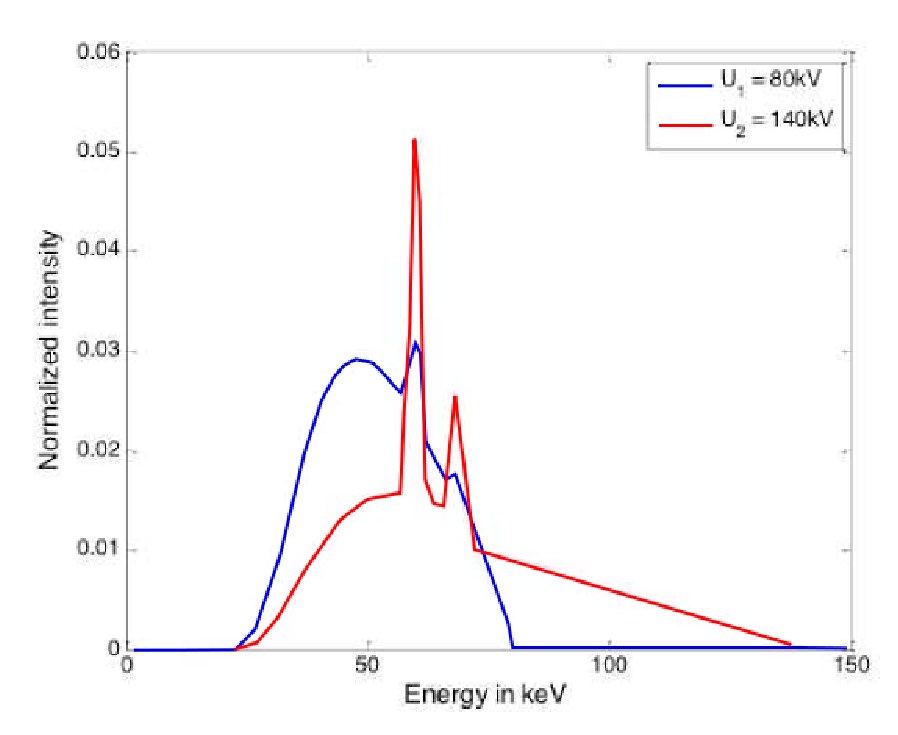
\includegraphics[height=160px]{images/dual1.eps} & 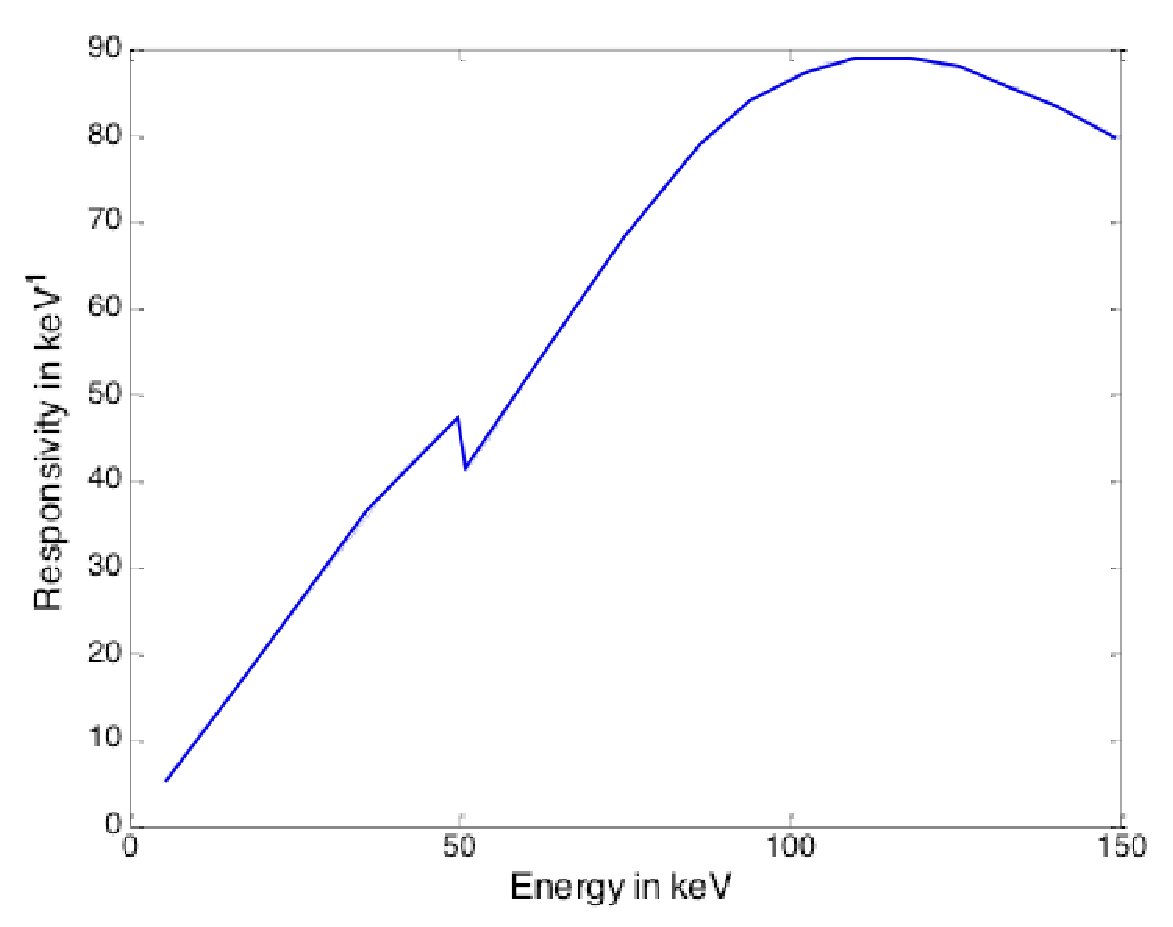
\includegraphics[height=160px]{images/dual2.eps} & 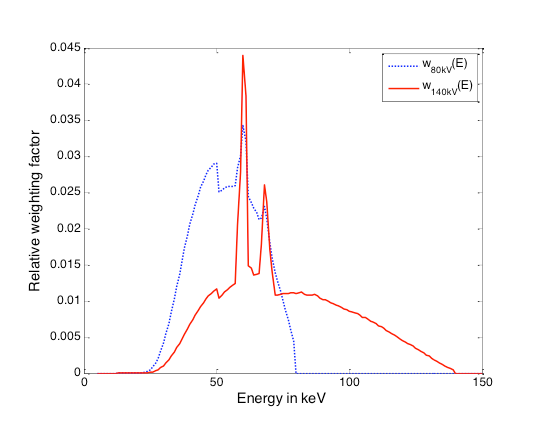
\includegraphics[height=160px]{images/dual3.eps} \\
    %{\large Normalized tube spectra S(E)}            & {\large Detector sensitivity D(E)}               & {\large Resulting system weighting functions}\end{tabular}
    %\end{center}
\end{frame}


\begin{frame}
    \frametitle{Dual Source CT}
    \begin{itemize}
        \item Two tube-detector setups in one gantry
        \item \bluefat{Pros:} Fast, system can be used for very fast single energy scans as well, commercially available
        \item \bluefat{Cons:} expensive, scatter radiation from system A to B and vice versa
    \end{itemize}
    \begin{figure}
        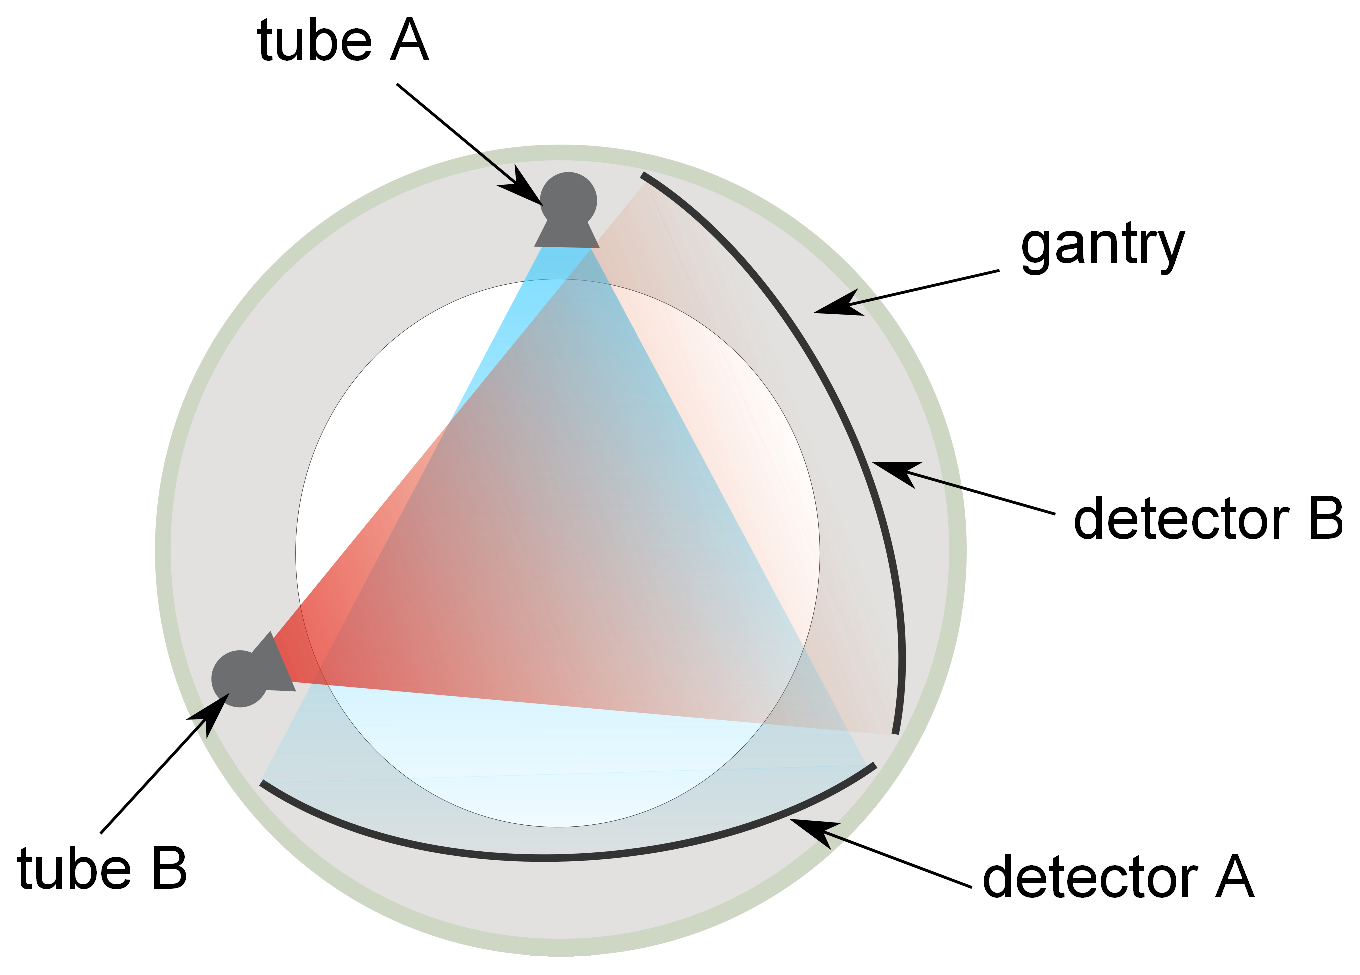
\includegraphics[height=0.6\textheight]{images/duals.eps}
    \end{figure}
\end{frame}

\begin{frame}
    \frametitle{Dual Layer Detectors}
    \begin{itemize}
        \item Two stacked scintillation detector layers
        \item \bluefat{Pros:} Fast, measurements are perfectly aligned
        \item \bluefat{Cons:} difficult hardware setup, weak separation between energy weightings
    \end{itemize}
    \begin{figure}
        \centering{}
        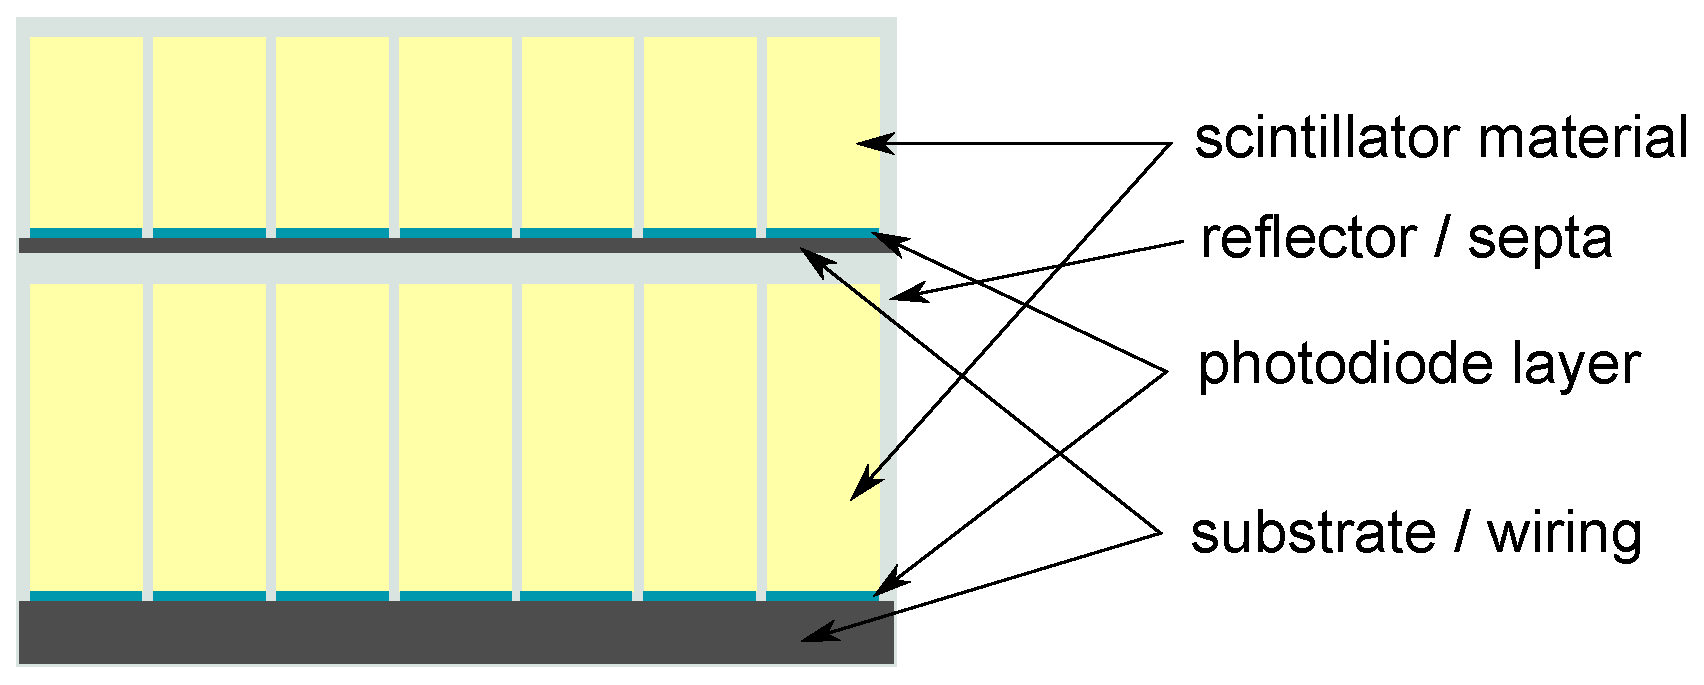
\includegraphics[height=0.6\textheight]{images/duall.eps}
    \end{figure}
\end{frame}

\begin{frame}[c]{Counting Detectors}
    \begin{itemize}
        \setlength\itemsep{0.4cm}

        \item Two principles: ``Optical counting'' with scintillators and counting direct converters
        \item The interactions between incoming X-ray photons and the detector material are converted into an electrical signal
        \item The electrical signal is sampled and quantized and then processed by an ASIC (application specific integrated circuit)
        \item Discriminator counts interaction events above given energy thresholds
    \end{itemize}
    %\begin{minipage}{0.4\textwidth}
    %\begin{figure}
    %{\large Detector layout of a direct converter}\\
    %\includegraphics[scale=.8]{images/count.eps}
    %\end{figure}
    %\end{minipage}
\end{frame}

\begin{frame}[c]{Counting Detectors}
    %\begin{minipage}{0.52\textwidth}
    \begin{itemize}
        \setlength\itemsep{0.4cm}
        \item Multiple thresholds yield multiple measurements at different energy levels
        \item \bluefat{Pros:} Fast, measurements are perfectly aligned
        \item \bluefat{Cons:} Pile-up of pulses at high X-ray flux, separation of energy weightings is limited by physical phenomena, further research needed to overcome limitations of semi-conductor material
    \end{itemize}
    %\end{minipage}
    %\begin{minipage}{0.42\textwidth}
    %\begin{center}
    %{\small Courtesy of Dr. Daniel Niederlöhner, Siemens Healthcare CT}\\
    %\includegraphics[height=180px]{images/counting.eps} \\
    %{\large Signal example of a directly converting detector that illustrates the discrimination thresholds and counted events}
    %\end{center}
    %\end{minipage}
\end{frame}

\begin{frame}[c]{Decomposition of Spectral Attenuation Coefficients}
    \begin{itemize}
        \item Various decompositions for the spectral attenuation coefficient exist
              \begin{itemize}
                  \item Photoelectric effect and incoherent (Compton) scatter component
                  \item Basis material components (e.g.\ mass attenuation of water and bone)
              \end{itemize}
        \item The basis material decomposition for two materials $a$ and $b$ reads:
              \begin{eqnarray*}
                  \mu(E, \vec x) = \rho_a(\vec x)\phi_a (E) + \rho_b(\vec x)\phi_b (E)
              \end{eqnarray*}
        \item This decomposition separates the energy dependent mass attenuation basis function $\phi(E)=\left(\frac{\mu}{\rho}\right)(E)$ from the spatially dependent effective basis material density  coefficient $\rho(\vec x)$
    \end{itemize}
\end{frame}

\begin{frame}[c]{Basis Material Decomposition}
    \begin{itemize}
        \setlength\itemsep{0.3cm}
        \item This property can be used together with the polychromatic attenuation formula to compute the basis material densities $\rho_a(\vec x)$ and  $\rho_b(\vec x)$ from multiple measurements at different spectral weightings
        \item This can either be done in the projection domain or in the image domain
        \item The latter approach requires the incorporation of a physically correct beam hardening model
        \item Both methods require lots of additional steps
        \item Please refer to the literature sources for practical realizations
    \end{itemize}
\end{frame}

\begin{frame}[t]{Material Decomposition}
	\begin{figure}[htpb]
		\centering
		\includegraphics[height=0.75\textheight]{images/lu_material_decomposition.png}
		\caption{Simulated projection images of a material decomposition.}%
	\end{figure}
	\vspace{-0.5cm}
	\flushright{}
	\tiny
	\fullcite{lu_material_decomposition}
\end{frame}

\begin{frame}[c]{Material Decomposition}
	\begin{figure}[htpb]
		\centering
		\includegraphics[height=0.55\textheight]{images/lu_material_decompositon2.png}
		\caption{Estimated material decomposition using a machine learning algorithm.}%
	\end{figure}
	\flushright{}
	\tiny
	\fullcite{lu_material_decomposition}
\end{frame}

\begin{frame}[t]{Material Decomposition}
	\vspace{-1cm}
	\begin{figure}[htpb]
		\centering
		\includegraphics[height=0.8\textheight]{images/mueller_material_decomposition1.png}
		\caption{Measured energy decomposition with two energy bins. LE:\ low energy bin, HE:\ high energy bin, TE:\ total energy.}%
	\end{figure}
	\flushright{}
	\tiny
	\fullcite{mueller_material_decomposition}
\end{frame}

\begin{frame}[t]{Material Decomposition}
	\begin{figure}[htpb]
		\centering
		\includegraphics[height=0.6\textheight]{images/mueller_material_decomposition2.png}
		\caption{Patches of the different techniques to extract iodinated contrasted vessel from background and respective signal to noise ratio.}%
	\end{figure}
	\flushright{}
	\tiny
	\fullcite{mueller_material_decomposition}
\end{frame}


\begin{frame}[t]{Material Decomposition}
	\begin{figure}[htpb]
		\centering
		\includegraphics[height=0.7\textheight]{images/dorn_dual_energy.png}
		\caption{Context-sensitive dual energy evaluation scheme. Each of the applications is automatically invoked and applied to the organ of interest.}%
	\end{figure}
	\flushright{}
	\tiny
	\fullcite{dorn18_dual_energy}
\end{frame}


\section{Take Home Messages}

\begin{frame}
    \frametitle{Take Home Messages}
    \begin{itemize}
        \item Beam hardening
        \item Spectral CT
        \item Base material decomposition
        \item Different measurement approaches
    \end{itemize}
\end{frame}


\section{Further Readings}

\begin{frame}
    \frametitle{Further Readings}
    \begin{itemize}
        \setlength\itemsep{0.4cm}

        \item \fullcite{taubmann18}

        \item Mass attenuation database (XCOM) \\
              {\large{\url{http://physics.nist.gov/PhysRefData/Xcom/html/xcom1.html}}}
        \item Balda, Michael: \textit{Quantitative Computed Tomography} (Dissertation); Pattern Recognition Lab, University of Erlangen-Nürnberg, Germany, 2011. \\
              {\large{\url{http://www5.informatik.uni-erlangen.de/Forschung/Publikationen/2011/Balda11-QCT.pdf}}}


    \end{itemize}
\end{frame}


\end{document}


